\section{CNNs and ImageNet}

% Slide 14 - Meet Yann LeCun
\begin{frame}{Meet Yann LeCun}
    \begin{columns}
        \column{0.4\textwidth}
        % TODO: Add photo
        % 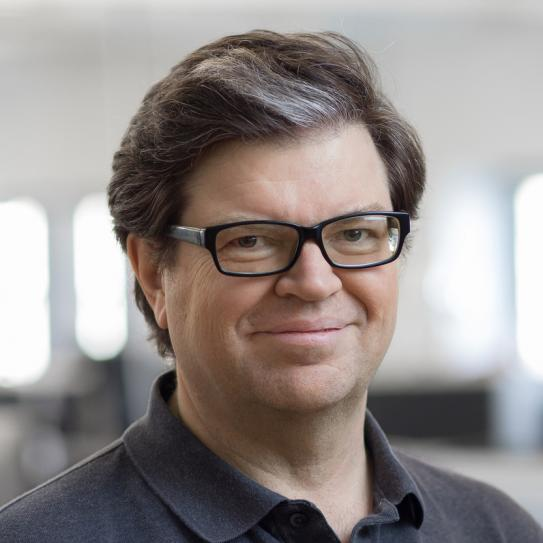
\includegraphics[width=\textwidth]{figures/lecun}
        
        \column{0.6\textwidth}
        \begin{itemize}
            \item \textbf{Invented CNNs} (LeNet)
            \item Bank check recognition system
            \item Reading \textbf{10\% of all US checks} by late 1990s
        \end{itemize}
    \end{columns}
    
    \vspace{1em}
    \textit{``Another author. Another invention we're about to explain.''}
\end{frame}

% Slide 15 - What is a CNN?
\begin{frame}{What is a CNN?}
    \textbf{The problem:} Standard networks ignore spatial structure
    
    \vspace{1em}
    \textbf{The solution:} Convolutional Neural Networks
    \begin{itemize}
        \item Convolution layers - detect local features
        \item Pooling layers - reduce spatial dimensions
        \item Feature maps - hierarchical representations
    \end{itemize}
    
    \vspace{1em}
    \textbf{Biologically inspired} - mirrors the visual cortex
    
    % TODO: Add CNN diagram
\end{frame}

% Slide 16 - How CNNs are Trained
\begin{frame}{How CNNs are Trained}
    % TODO: Add visualization of learned filters
    
    \begin{quote}
        ``When ConvNet models and monkeys are shown the same picture, the activations of high-level units in the ConvNet explains half of the variance of random sets of 160 neurons in the monkey's inferotemporal cortex.''
    \end{quote}
    
    \vspace{1em}
    \textbf{They're not just saying it works - they're saying it works like a brain.}
\end{frame}

% Slide 17 - Early CNN Deployments
\begin{frame}{Early CNN Deployments}
    \begin{itemize}
        \item Speech recognition, OCR, handwriting recognition
        \item Microsoft deployments
        \item Face and hand detection in the early 90s
    \end{itemize}
    
    \vspace{1em}
    \textbf{``This was working for 20 years and the mainstream ignored it.''}
\end{frame}

% Slide 18 - ImageNet 2012
\begin{frame}{ImageNet 2012}
    \textbf{AlexNet enters the competition}
    
    \vspace{1em}
    \begin{itemize}
        \item \textbf{Almost halving} error rates of the best competing approach
        \item Key ingredients:
        \begin{itemize}
            \item GPUs
            \item ReLU activation
            \item Dropout regularization
            \item Data augmentation
        \end{itemize}
    \end{itemize}
    
    \vspace{1em}
    \textbf{This is the moment the mainstream could no longer ignore it.}
\end{frame}

% Slide 19 - The World Notices
\begin{frame}{The World Notices}
    \begin{quote}
        ``Companies such as Mobileye and NVIDIA are using such ConvNet-based methods in their upcoming vision systems for cars.''
    \end{quote}
    
    \vspace{1em}
    \begin{itemize}
        \item NVIDIA investing in deep learning chips
        \item Tesla self-driving cars
        \item \textit{If you read this paper in 2015 and bought NVIDIA stock...}
    \end{itemize}
    
    \vspace{1em}
    \textbf{The hype is warranted - they know it's going to work.}
\end{frame}

% Slide 20 - Why Was it Ignored for So Long?
\begin{frame}{Why Was it Ignored for So Long?}
    \begin{itemize}
        \item CNNs were largely forsaken until 2012
        \item \textbf{Despite working since the early 90s}
        \item The AI winters left scars
    \end{itemize}
    
    \vspace{1em}
    \textit{``If it works for images, what about language?''}
\end{frame}
